% ta med damping på DP-delle

\documentclass[aspectratio=169,xcolor=dvipsnames]{beamer}
%\usetheme{SimplePlus}

\usepackage{hyperref}
\usepackage{graphicx} % Allows including images
\usepackage{booktabs} % Allows the use of \toprule, \midrule and \bottomrule in tables

%----------------------------------------------------------------------------------------
%	TITLE PAGE
%----------------------------------------------------------------------------------------

\title[Industrielektronikk]{Industrielektronikk} % The short title appears at the bottom of every slide, the full title is only on the title page
%\subtitle{Subtitle}

\author[Fred-Olav] {Fred-Olav Mosdal}

\institute[Gand VGS] % Your institution as it will appear on the bottom of every slide, may be shorthand to save space
{
    Gand VGS \\
    VG1 TIF }
\date{\today} % Date, can be changed to a custom date


%----------------------------------------------------------------------------------------
%	PRESENTATION SLIDES
%----------------------------------------------------------------------------------------

\begin{document}
\begin{frame}
\titlepage
\end{frame}

\begin{frame}
	\frametitle{Styringsteknikk D426}

	\begin{columns}
		\begin{column}{0.5\textwidth}
			Mål:
			\begin{itemize}
				\item \url{https://www.udir.no/lk20/pin02-03}
			\end{itemize}
		\end{column}

		\begin{column}{0.5\textwidth}
			$$\includegraphics[width=0.8\textwidth]{../output/noGPLimages/udir.pdf}$$
		\end{column}
	\end{columns}
\end{frame}

\begin{frame}
	\frametitle{Fagenes relevans og sentrale verdier}

	\begin{columns}
		\begin{column}{0.5\textwidth}
			Vg2 industriteknologi handler om å utvikle kompetanse innenfor teknologiske, produksjonsrettede og utviklingsorienterte yrker. Programfagene gir en bred plattform for videre yrkesvalg innenfor bruk av ulike materialer, verktøy, teknikker og maskiner. Programfagene skal bidra til å utvikle elevene til selvstendige og omstillingsdyktige fagarbeidere innenfor yrker der programmering, robotisering og automatisering er en del av hverdagen. Programfagene skal bidra til å utvikle en helhetsforståelse av produksjonsprosesser og gi en tverrfaglig forståelse av fagområdene i arbeidslivet.
		\end{column}

		\begin{column}{0.5\textwidth}
			$$\includegraphics[width=0.8\textwidth]{../output/noGPLimages/udir.pdf}$$
		\end{column}
	\end{columns}
\end{frame}

\begin{frame}
	\frametitle{Kompetansemål:}

	\begin{columns}
		\begin{column}{0.5\textwidth}
			Mål:
			\begin{itemize}
				
				\item montere, sette i drift og feilsøke maskiner og utstyr i en produksjonsprosess
				\item montere, sette i drift og feilsøke automatiserte hydraulikk- og pneumatikkanlegg etter spesifikasjoner 
				\item planlegge og gjennomføre praktiske arbeidsoppgaver i både kjente og ukjente sammenhenger 
				\item bruke digitale verktøy til å utarbeide modeller, tegninger, skjemaer, arbeidsbeskrivelser og kvalitetssikringssystemer i planlegging og produksjon 

			\end{itemize}
		\end{column}

		\begin{column}{0.5\textwidth}
			$$\includegraphics[width=0.8\textwidth]{../output/noGPLimages/udir.pdf}$$
		\end{column}
	\end{columns}
\end{frame}
\begin{frame}
	\frametitle{Kompetansemål:}

	\begin{columns}
		\begin{column}{0.5\textwidth}
			Mål:
			\begin{itemize}
				\item utarbeide rapporter og skjemaer knyttet til arbeidsoppgaver og vurdere resultatet av eget arbeid 
				\item anvende program for simulering og styring av robot og automasjon 
				\item bruke additiv tilvirkning for å løse læringsoppdrag 
				\item utarbeide og følge sikker jobb-analyser ved farlige operasjoner i henhold til gjeldende forskrifter 
				\item arbeide på elektriske og automatiserte systemer ved reparasjons- og vedlikeholdsarbeid etter instrukser og gjeldende forskrifter

			\end{itemize}
		\end{column}

		\begin{column}{0.5\textwidth}
			$$\includegraphics[width=0.8\textwidth]{../output/noGPLimages/udir.pdf}$$
		\end{column}
	\end{columns}
\end{frame}

\begin{frame}
	\frametitle{Boken}

	\begin{columns}
		\begin{column}{0.5\textwidth}
			I styringsteknikken skal vi ha følgende kapittel:

			\begin{itemize}
			\item Kap. 11 Programmerbare logiske styringer 
			\item Kap. 12 Elektriske Anlegg 
			\item Kap. 13 Hydraulikk 
			\item Kap. 14 Pneumatikk

			\end{itemize}
		\end{column}

		\begin{column}{0.5\textwidth}
			$$\includegraphics[width=0.7\textwidth]{../output/noGPLimages/RepOgVedlikehold.jpg}$$
		\end{column}
	\end{columns}
\end{frame}

\begin{frame}
	\frametitle{Grunnkunnskaper}

	\Huge
	Grunnkunnskaper\\
\normalsize
\vskip 2 cm
Kunnskaper som må være på plass for å forstå det som kommer
\end{frame}


\begin{frame}
	\frametitle{SI-prefikser}

	\begin{columns}
		\begin{column}{0.5\textwidth}
			Mål:
			\begin{itemize}
				\item Brukes ved store eller små strørrelser 
				\item Hardisk på 2TB
				\item Prosessor med transistorstørrelse på 7nm
			\end{itemize}
		\end{column}

		\begin{column}{0.5\textwidth}
			$$\includegraphics[width=0.8\textwidth]{SIenheter.eps}$$
		\end{column}
	\end{columns}
\end{frame}


\begin{frame}
	\frametitle{Atomstrukturen}

	\begin{columns}
		\begin{column}{0.5\textwidth}
			\begin{itemize}
				\item Protorner, nøytroner og elektroner 
				\item Antall elektroner i yterste skallet avgjør elektriske egenskaper
	\item Metaller. Dette er materialer som leder godt. De har 1-3 elektroner i valensskallet. Disse er forholdsvis løst bundet til atomet. Vi sier	da at det har mange frie elektroner. 
	\item Halvledere. Materialer som ikke leder like godt som metaller. Det	har noen unike egenskaper. Disse egenskapene gjør at vi kan bruke det til å lage dioder, transistorer og CPU-er.
	\item Isolatorer. Materialer som leder dårlig. Disse brukes der vi ikke	vil at det skal gå strøm. 
			\end{itemize}
		\end{column}

		\begin{column}{0.5\textwidth}
			$$\includegraphics[width=0.8\textwidth]{./chemistry17.eps}$$
		\end{column}
	\end{columns}
\end{frame}

\begin{frame}
	\frametitle{Elektrisk ladning}

	\begin{columns}
		\begin{column}{0.5\textwidth}
			Tekst
			\begin{itemize}
				\item Et eksempel er statisk elektrisitet. 
				\item Kjemisk reaksjon i et batteri. 
				\item Roterende magnestisk felt i en generator
			\end{itemize}
		\end{column}

		\begin{column}{0.5\textwidth}
			$$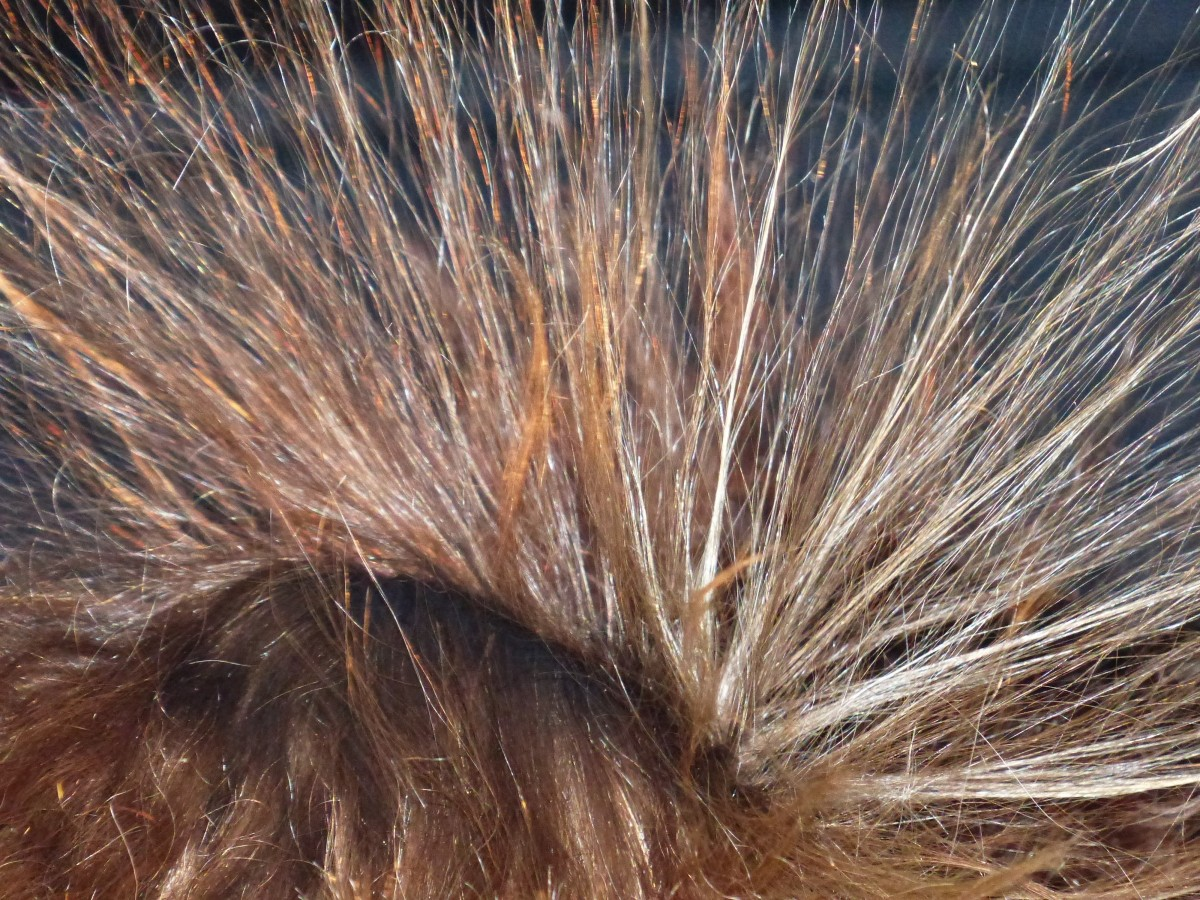
\includegraphics[width=1\textwidth]{./hair_van_de_graaf_generator.jpg}$$
		\end{column}
	\end{columns}
\end{frame}

\begin{frame}
	\frametitle{Spenning, Strøm og Resistans}

			$$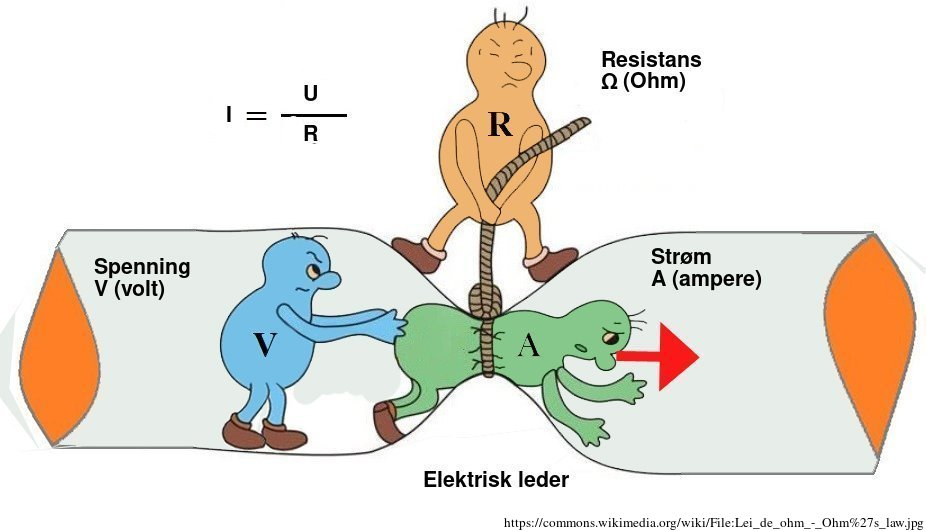
\includegraphics[width=0.9\textwidth]{./ohmslov.jpg}$$
\end{frame}

\begin{frame}
	\frametitle{Spenningskilder}

	\begin{columns}
		\begin{column}{0.5\textwidth}
			\begin{itemize}
				\item Batteri 
				\item Strømforsyning 
				\item Uttak i veggen 
				\item ...
			\end{itemize}
		\end{column}

		\begin{column}{0.5\textwidth}
%			$$\includegraphics[width=0.8\textwidth]{SIenheter.eps}$$
		\end{column}
	\end{columns}
\end{frame}

\begin{frame}
	\frametitle{En Enkel Krets}

			$$
\includegraphics[width=0.8\textwidth]{./eksempel1.pdf}$$
\end{frame}


\begin{frame}
	\frametitle{Eksempel 1}

	\begin{columns}
		\begin{column}{0.5\textwidth}
Hvor mange ampere går det i kretsen på figuren
		\end{column}

		\begin{column}{0.5\textwidth}
			$$
\includegraphics[width=1\textwidth]{./eksempel1.pdf}$$
		\end{column}
	\end{columns}
\end{frame}

\begin{frame}
	\frametitle{Eksempel 1}

	\begin{columns}
		\begin{column}{0.5\textwidth}
Hvor mange ampere går det i kretsen på figuren
\vskip 1cm
Løsning: Bruker formelen $I=\dfrac{U}{R}$

\[
I=\dfrac{U}{R}=\dfrac{100V}{22\Omega}=\underline{\underline{4.6A}}
\]
\vskip 1cm
Lignende problem: Hva blir strømmen om R forandres til 33$\Omega$
i kretsen på figuren
		\end{column}

		\begin{column}{0.5\textwidth}
			$$
\includegraphics[width=0.8\textwidth]{./eksempel1.pdf}$$
		\end{column}
	\end{columns}
\end{frame}



\begin{frame}
	\frametitle{Eksempel 2}

	\begin{columns}
		\begin{column}{0.5\textwidth}
			Hvis resistansen i figuren forandres til 47$\Omega$ og
spenningen til 50v, hva blir strømmen?


		\end{column}

		\begin{column}{0.5\textwidth}
			$$
\includegraphics[width=0.8\textwidth]{./eksempel1.pdf}$$
		\end{column}
	\end{columns}
\end{frame}


\begin{frame}
	\frametitle{Eksempel 2}

	\begin{columns}
		\begin{column}{0.5\textwidth}
			Hvis resistansen i figuren forandres til 47$\Omega$ og
spenningen til 50v, hva blir strømmen?

\vskip 0.5cm
Løsning: Erstatter U=50V og R=47$\Omega$ i formelen $I=\dfrac{U}{R}$

\[
I=\dfrac{U}{R}=\dfrac{50V}{47\Omega}=\underline{\underline{1.1A}}
\]

Lignende problem: Hvis U=5V og R=1000$\Omega$, hva blir strømmen?

		\end{column}

		\begin{column}{0.5\textwidth}
			$$
\includegraphics[width=0.8\textwidth]{./eksempel1.pdf}$$
		\end{column}
	\end{columns}
\end{frame}

\begin{frame}
	\frametitle{Eksempel 3}

	\begin{columns}
		\begin{column}{0.5\textwidth}
Finn strømmen 
		\end{column}

		\begin{column}{0.5\textwidth}
			$$\includegraphics[width=0.8\textwidth]{./Eksempel3.pdf}$$
		\end{column}
	\end{columns}
\end{frame}
\begin{frame}
	\frametitle{Eksempel 3}

	\begin{columns}
		\begin{column}{0.5\textwidth}
Finn strømmen 
\vskip 1cm
Løsning: Husk at 1.0k$\Omega$ er det samme som $1\cdot10^{3}\Omega$.
Bruk formelen $I=\dfrac{U}{R}$

\[
I=\dfrac{U}{R}=\dfrac{50V}{1.0k\Omega}=\dfrac{50V}{1.0\cdot10^{3}}=\underline{\underline{50mA}}
\]
		\end{column}

		\begin{column}{0.5\textwidth}
			$$\includegraphics[width=0.8\textwidth]{./Eksempel3.pdf}$$
		\end{column}
	\end{columns}
\end{frame}


\begin{frame}
	\frametitle{Eksempel 4}

	\begin{columns}
		\begin{column}{0.5\textwidth}
Hvor mange milliampere går det i kretsen på figuren 
		\end{column}

		\begin{column}{0.5\textwidth}
			$$\includegraphics[width=0.8\textwidth]{./Eksempel4.pdf}$$
		\end{column}
	\end{columns}
\end{frame}

\begin{frame}
	\frametitle{Eksempel 4}

	\begin{columns}
		\begin{column}{0.5\textwidth}
Hvor mange milliampere går det i kretsen på figuren 
\vskip 0.5cm
Løsning: Bruk formelen $I=\dfrac{U}{R}$

\[
I=\dfrac{U}{R}=\dfrac{30V}{5.6k\Omega}=\dfrac{30V}{5.6\cdot10^{3}}=\underline{\underline{5.4mA}}
\]
		\end{column}

		\begin{column}{0.5\textwidth}
			$$\includegraphics[width=0.8\textwidth]{./Eksempel4.pdf}$$
		\end{column}
	\end{columns}
\end{frame}
\begin{frame}
	\frametitle{Bruk av multimeter i enkel krets for å måle spenning}

	\begin{columns}
		\begin{column}{0.3\textwidth}
\begin{itemize}
	\item Multimeteret stilles på rett område for å måle likespenning 
	\item Måleledningene kobles over motstanden vi ønsker å finne spenningen over.
\end{itemize}
		\end{column}

		\begin{column}{0.7\textwidth}
			$$\includegraphics[width=1\textwidth]{./pIndustrielektronikk01.eps}$$
		\end{column}
	\end{columns}
\end{frame}

\begin{frame}
	\frametitle{Bruk av multimeter i enkel krets for å måle strøm}

	\begin{columns}
		\begin{column}{0.3\textwidth}
\begin{itemize}
	\item Multimeteret stilles på rett område for å måle likestrøm 
	\item Måleledningene kobles i serie med motstanden vi ønsker å finne strømmen igjennom.
	\item NB. om vi kobler feil ved strømmåling kan vi lage en kortsluttning. 
\end{itemize}
		\end{column}

		\begin{column}{0.7\textwidth}
			$$\includegraphics[width=1\textwidth]{./pIndustrielektronikk02.eps}$$
		\end{column}
	\end{columns}
\end{frame}
\begin{frame}
	\frametitle{Bruk av multimeter i enkel krets for å måle motstanden}

	\begin{columns}
		\begin{column}{0.3\textwidth}
\begin{itemize}
	\item Multimeteret stilles på rett område for å måle motstand 
	\item Kretsen kobles fa spenningskilden
	\item Måleledningene kobles over motstanden vi ønsker å finne motstanden i.
\end{itemize}
		\end{column}

		\begin{column}{0.7\textwidth}
			$$\includegraphics[width=1\textwidth]{./pIndustrielektronikk03.eps}$$
		\end{column}
	\end{columns}
\end{frame}
\begin{frame}
	\frametitle{Seriekretser}

	\begin{columns}
		\begin{column}{0.5\textwidth}
I en seriekrets kobles flere komponenter etter hverandre. I en slik
krets har strømmen en vei å gå. Vi kan derfor si at strømmen er den
samme overalt i en serie krets. 

Spenninen som påtrykkes seriekretsen vil fordeles seg over motstandene
etter Kirchhoff's spenningslov:
\[
U_{t}=U_{1}+U_{2}+U_{3}+......+U_{n}
\]

Eller med ord: Summen av alle spenninger i en seriekrets er null.

		\end{column}

		\begin{column}{0.5\textwidth}

Total resistansen i en seriekrets finner vi ved å legge sammen alle
motstandere:
\[
R_{t}=R_{1}+R_{2}+R_{3}+......+R_{n}
\]

Tegn opp motstandere i flere mønster som skal kobles i serie.
		\end{column}
	\end{columns}
\end{frame}


\begin{frame}
	\frametitle{Bruk av multimeter i seriekretser for å måle spenning}

	\begin{columns}
		\begin{column}{0.3\textwidth}
\begin{itemize}
	\item Multimeteret stilles på rett område for å måle likespenning 
	\item Måleledningene kobles over motstanden vi ønsker å finne spenningen over, her motstanden på 3k3. 
\end{itemize}
		\end{column}

		\begin{column}{0.7\textwidth}
			$$\includegraphics[width=1\textwidth]{./pIndustrielektronikk04.eps}$$
		\end{column}
	\end{columns}
\end{frame}

\begin{frame}
	\frametitle{Bruk av multimeter i seriekretser for å måle spenning}

	\begin{columns}
		\begin{column}{0.3\textwidth}
\begin{itemize}
	\item Multimeteret stilles på rett område for å måle likespenning 
	\item Måleledningene kobles over motstanden vi ønsker å finne spenningen over her motstanden på 2k2.
\end{itemize}
		\end{column}

		\begin{column}{0.7\textwidth}
			$$\includegraphics[width=1\textwidth]{./pIndustrielektronikk05.eps}$$
		\end{column}
	\end{columns}
\end{frame}

\begin{frame}
	\frametitle{Bruk av multimeter i seriekretser for å måle strøm}

	\begin{columns}
		\begin{column}{0.3\textwidth}
\begin{itemize}
	\item Multimeteret stilles på rett område for å måle likestrøm 
	\item Måleledningene kobles i serie med kretsen
\end{itemize}
		\end{column}

		\begin{column}{0.7\textwidth}
			$$\includegraphics[width=1\textwidth]{./pIndustrielektronikk06.eps}$$
		\end{column}
	\end{columns}
\end{frame}

\begin{frame}
	\frametitle{Bruk av multimeter i seriekretser for å måle total motstand}

	\begin{columns}
		\begin{column}{0.3\textwidth}
\begin{itemize}
	\item Multimeteret stilles på rett område for å måle omtstand 
	\item Kretsen kobles fra strømforsyningen
	\item Måleledningene kobles over kretsen
\end{itemize}
		\end{column}

		\begin{column}{0.7\textwidth}
			$$\includegraphics[width=1\textwidth]{./pIndustrielektronikk07.eps}$$
		\end{column}
	\end{columns}
\end{frame}
\begin{frame} \frametitle{Parallellkretser}
	\begin{columns}
		\begin{column}{0.5\textwidth}
			I en parallellkrets er flere komponenter koblet til to punkter(noder).
Dette gjør at spenningen er lik over alle motstandere i en paralellkobling.
Stømmen igjennom en motstand i paralellkobling blir da $I=\dfrac{U}{R_{en\,eller\,annen}}$.
Summen av alle strømmer i paralellkoblingen blir det vi kaller hovedstrømmen:

\[
I_{t}=I_{1}+I_{2}+I_{3}+......+I_{n}
\]

		\end{column}
		\begin{column}{0.5\textwidth}
Resisansen i en paralellkobling:

\[
R_{t}=\dfrac{1}{\dfrac{1}{R_{1}}+\dfrac{1}{R_{2}}+\dfrac{1}{R_{3}}+......+\dfrac{1}{R_{n}}}
\]

		\end{column}
	\end{columns}
\end{frame}
\begin{frame}
	\frametitle{Bruk av multimeter i parallellkretser for å måle spenning}

	\begin{columns}
		\begin{column}{0.3\textwidth}
\begin{itemize}
	\item Multimeteret stilles på rett område for å måle spenning 
	\item Måleledningene kobles over parallellkoblingen
\end{itemize}
		\end{column}

		\begin{column}{0.7\textwidth}
			$$\includegraphics[width=1\textwidth]{./pIndustrielektronikk08.eps}$$
		\end{column}
	\end{columns}
\end{frame}
\begin{frame}
	\frametitle{Bruk av multimeter i parallellkretser for å måle 1. grenstrøm}

	\begin{columns}
		\begin{column}{0.3\textwidth}
\begin{itemize}
	\item Multimeteret stilles på rett område for å måle strøm 
	\item Måleledningene kobles i serie med den ene grenen av parallellkoblingen 
\end{itemize}
		\end{column}

		\begin{column}{0.7\textwidth}
			$$\includegraphics[width=1\textwidth]{./pIndustrielektronikk09.eps}$$
		\end{column}
	\end{columns}
\end{frame}
\begin{frame}
	\frametitle{Bruk av multimeter i parallellkretser for å måle 2. grenstrøm}

	\begin{columns}
		\begin{column}{0.3\textwidth}
\begin{itemize}
	\item Multimeteret stilles på rett område for å måle strøm 
	\item Måleledningene kobles i serie med den andre grenen av parallellkoblingen 
\end{itemize}
		\end{column}

		\begin{column}{0.7\textwidth}
			$$\includegraphics[width=1\textwidth]{./pIndustrielektronikk10.eps}$$
		\end{column}
	\end{columns}
\end{frame}
\begin{frame}
	\frametitle{Bruk av multimeter i parallellkretser for å måle hovedstrøm}

	\begin{columns}
		\begin{column}{0.3\textwidth}
\begin{itemize}
	\item Multimeteret stilles på rett område for å måle strøm 
	\item Måleledningene kobles i serice med parallellkoblingen
\end{itemize}
		\end{column}

		\begin{column}{0.7\textwidth}
			$$\includegraphics[width=1\textwidth]{./pIndustrielektronikk11.eps}$$
		\end{column}
	\end{columns}
\end{frame}
\begin{frame}
	\frametitle{Bruk av multimeter i parallellkretser for å måle resistans}

	\begin{columns}
		\begin{column}{0.3\textwidth}
\begin{itemize}
	\item Multimeteret stilles på rett område for å måle resistans
	\item Kretsen kobles fra strømforsyningen
	\item Måleledningene kobles over kretsen
\end{itemize}
		\end{column}

		\begin{column}{0.7\textwidth}
			$$\includegraphics[width=1\textwidth]{./pIndustrielektronikk12.eps}$$
		\end{column}
	\end{columns}
\end{frame}


\begin{frame} \frametitle{Kombinerte kretser}
	\begin{columns}
		\begin{column}{0.5\textwidth}
			
Ofte finner en kretser med en kombinasjon av seriekobling og parallellkobling. Utfordringen ligger i å finne hva som er koblet i serie og hva som er koblet i parallell. 
		\end{column}
		\begin{column}{0.5\textwidth}
			$$\includegraphics[width=0.8\textwidth]{./kombieks1.pdf}$$
		\end{column}
	\end{columns}
\end{frame}

\begin{frame} \frametitle{Kombinerte kretser}
	\begin{columns}
		\begin{column}{0.5\textwidth}
			

I figuren kan vi se at $R_{1}$
er i serie med parallellkoblingen av $R_{2}$ og $R_{3}$. Dette kan
vi skrive som:
\[
R_{1}+R_{2}||R_{3}
\]

Om vi vil kan vi erstatte $R_{2}||R_{3}$med en $R_{p}$. Vi har da
en serie kobling av $R_{1}+R_{p}$ 
		\end{column}
		\begin{column}{0.5\textwidth}
			$$\includegraphics[width=0.8\textwidth]{./kombieks1.pdf}$$
		\end{column}
	\end{columns}
\end{frame}

\begin{frame} \frametitle{Kombi eksempel}
	\begin{columns}
		\begin{column}{0.5\textwidth}
Prøv å finne ut hvilke motstandere som er i serie og parallell i denne
kretsen:


		\end{column}
		\begin{column}{0.5\textwidth}
			\includegraphics[width=0.9\textwidth]{./kombieks2.pdf}
		\end{column}
	\end{columns}
\end{frame}
\begin{frame}\frametitle{Bruk av multimeter i kombikretser for å måle spenning}

	\begin{columns}
		\begin{column}{0.3\textwidth}
\begin{itemize}
	\item Multimeteret stilles på rett område for å måle spenning
	\item Måleledningene kobles over motstandene vi skal finne spenningen over
\end{itemize}
		\end{column}

		\begin{column}{0.7\textwidth}
			$$\includegraphics[width=1\textwidth]{./pIndustrielektronikk13.eps}$$
		\end{column}
	\end{columns}
\end{frame}
\begin{frame}\frametitle{Bruk av multimeter i kombikretser for å måle spenning}

	\begin{columns}
		\begin{column}{0.3\textwidth}
\begin{itemize}
	\item Multimeteret stilles på rett område for å måle spenning
	\item Måleledningene kobles over motstandene vi skal finne spenningen over
\end{itemize}
		\end{column}

		\begin{column}{0.7\textwidth}
			$$\includegraphics[width=1\textwidth]{./pIndustrielektronikk14.eps}$$
		\end{column}
	\end{columns}
\end{frame}
\begin{frame}\frametitle{Bruk av multimeter i kombikretser for å måle spenning}

	\begin{columns}
		\begin{column}{0.3\textwidth}
\begin{itemize}
	\item Multimeteret stilles på rett område for å måle spenning
	\item Måleledningene kobles over motstandene vi skal finne spenningen over
\end{itemize}
		\end{column}

		\begin{column}{0.7\textwidth}
			$$\includegraphics[width=1\textwidth]{./pIndustrielektronikk15.eps}$$
		\end{column}
	\end{columns}
\end{frame}
\begin{frame}\frametitle{Bruk av multimeter i kombikretser for å måle strøm}

	\begin{columns}
		\begin{column}{0.3\textwidth}
\begin{itemize}
	\item Multimeteret stilles på rett område for å måle strøm
	\item Måleledningene kobles i serie grenstrømmen vi vil finne strømmen i 
\end{itemize}
		\end{column}

		\begin{column}{0.7\textwidth}
			$$\includegraphics[width=1\textwidth]{./pIndustrielektronikk16.eps}$$
		\end{column}
	\end{columns}
\end{frame}
\begin{frame}\frametitle{Bruk av multimeter i kombikretser for å måle strøm}

	\begin{columns}
		\begin{column}{0.3\textwidth}
\begin{itemize}
	\item Multimeteret stilles på rett område for å måle strøm
	\item Måleledningene kobles i serie grenstrømmen vi vil finne strømmen i 
\end{itemize}
		\end{column}

		\begin{column}{0.7\textwidth}
			$$\includegraphics[width=1\textwidth]{./pIndustrielektronikk17.eps}$$
		\end{column}
	\end{columns}
\end{frame}
\begin{frame}\frametitle{Bruk av multimeter i kombikretser for å måle strøm}

	\begin{columns}
		\begin{column}{0.3\textwidth}
\begin{itemize}
	\item Multimeteret stilles på rett område for å måle strøm
	\item Måleledningene kobles i serie grenstrømmen vi vil finne strømmen i 
\end{itemize}
		\end{column}

		\begin{column}{0.7\textwidth}
			$$\includegraphics[width=1\textwidth]{./pIndustrielektronikk18.eps}$$
		\end{column}
	\end{columns}
\end{frame}



\end{document}
